\section{数据流编程理论与模型在类脑计算中的应用}
\subsection{引言}
近年来,借鉴人脑信息处理模式和结构的类脑计算得到了长足发展。类脑计算中最常用的计算模型是脉冲神经网络(spiking neural network,SNN),结合SNN与深度神经网络(deep neural network,DNN)各自优势的相关研究工作[天机芯片,nature]也正逐渐展开。

SNN网络的执行过程具有事件驱动、异步并发、活动稀疏性等特点,直观上较为符合数据流执行模型的特点,因此以数据流编程理论与模型为指导,进行类脑计算的SNN网络软件仿真与硬件芯片优化设计是题中应有之义。

本章就以下几方面问题开展了研究介绍,第一是数据流模型启发下的支持DNN特性的通用SNN描述语言,该语言针对SNN与DNN相融合的研究趋势,扩展了目前较为主流的SNN描述语言PyNN,是其能够支持DNN的描述需求;第二是面向GPGPU的SNN模拟,;最后是基于数据流模型有效指导类脑芯片结构设计,包括两个主要内容,即数据流模型指导下的神经网络编译以及与该编译技术对应的基于RRAM(阻变存储器)交叉开关结构的可重构神经网络加速器设计。

(包括一张图给出这几个方面的层次关系)


\subsection{支持DNN特性的通用SNN描述语言(计划替换为该内容)}
(1)通用SNN描述语言的研究背景与动机\\
SNN是目前类脑计算采用的主要计算模型,DNN则是目前机器学习领域广泛应用的计算模型,随着双方研究工作的进展,SNN和DNN开始出现相互借鉴乃至逐步融合的趋势。SNN与DNN在神经元和突触模型、网络描述方式、信息传输模式和训练算法等方面存在的差异,使得现存的SNN描述语言并不支持DNN特性。因此一种通用 SNN 描述语言——支持DNN特性的SNN描述语言将在以下方面起到积极促进作用:

\begin{itemize}
    \item 训练算法:可以提高将DNN优秀的学习算法移植到SNN的效率。当前相关的工作往往要求使用者同时具有DNN(计算机和人工智能领域)和SNN(生物和脑科学领域)的相关背景,并能够熟练地使用两方面的相关工具。通用SNN描述语言可以减轻SNN开发人员对DNN相关背景知识和工具的依赖,使得他们在使用SNN同时,能够便捷地利用DNN领域的训练算法。
    \item 应用领域:目前,相当一部分神经形态芯片支持使用SNN语言进行应用开发(例如 BrainScaleS[8]和SpiNNaker[9]系统支持广泛使用的SNN描述语言PyNN[29])。通用SNN 描述语言可以将基于DNN的机器学习应用便捷地移 植到上述神经形态硬件平台,从而拓展上述硬件平台的应用领域。 
    \item 执行效率:部分神经形态芯片采用了异步电路设计以更加契合SNN的计算模型,从而极大地降低了芯片的功耗[30]。通用SNN描述语言有助于建立针对神经形态硬件的开发工具链,从而可以在上述平台上直接开发机器学习相 关应用,提高机器学习应用的执行性能并减少总体功耗。 
    \item 资源共享:尽管目前SNN和DNN相互借鉴甚至融合的趋势已经初步显现,但两者在神经元和突触模型、网络描述方式、训练算法,和信息传输模式层面的不同严重阻碍了双方社区的资源共享和互相合作。上述领域专用语言将有助于SNN共同体和DNN共同体的资源共享。

\end{itemize}

(2)SNN描述语言——PyNN\\

随着类脑计算的发展,出现了越来越多支持SNN 的计算平台,诸如SNN模拟器[11,12,15],神经形态芯片[8,9] 以及FPGA系统[32] 等。为提高SNN模型的可移植性和通用性,多种独立于模拟器的SNN描述语言(例如PyNN[29]和SpineML[51])得到了越来越广泛的应用。其中基于Python的领域专用语言PyNN,得到了众多 SNN模拟器(例如 NeMo[14],NEST[11],PCSIM[12],Brian[15]和Brian21 O[31])、众多神经形态芯片(例如BrainScaleS[8]和SpiNNaker[9])以及FPGA系统(例如NeuroFlow[32])的支持。通常情况下,PyNN 使用高层次的抽象模型(神经元组成的集群和它们之间的连接)描述SNN,提供了多种标准的神经元和突触模型,以及一系列的连接算法。

PyNN是一种基于Python的领域专用语言。用户可以使用PyNN构建基于Python代码的SNN模型,并可以在任意支持PyNN的模拟器上运行。PyNN的具体实现是一个由通用模块(包含标准的神经元、突触模型,以及一系列广泛使用的连接算法)和针对不同模拟器后端的专用模块组成的Python 包。PyNN 提供了一个面向对象的编程接口,可以在神经元集群和突触映射的层面描述 SNN。PyNN 的具体后端实现则可以将上层的 SNN 描述和底层模拟器实现的具体函数接口连接起来。因此,PyNN 语言本身仅仅提供了对 SNN 的高层次描述方法,具体的执行性能由后端实现决定。部分支持PyNN的模拟器实现(例如 Brian[15])通过代码生成来实现对使用PyNN描述的神经网络的高效执行。PyNN的核心语言类型如下:

\begin{itemize}
    \item 神经元类型。PyNN中所有的神经元类型都是类BaseCellType的子类。神经元对应的参数可以在实例化的同时进行设置,且不同的神经元模型都继承了相同的基本操作函数。PyNN中定义了多个常用的神经元类型(例如 IF\_curr\_exp, IF\_curr\_alpha等),这些神经元类型在不同的后端实现中都具有统一的计算实现。 PyNN中定义的神经元相应的计算类似 DNN 中的激活函数,PyNN 的原始定义中并没有提供对反向传播算法的支持。
    \item 集群。因为 PyNN 通常用于描述包含很多神经元的大规模 SNN,因此其默认使用多个相同类型的神经元组成的集群作为 SNN 描述的基本单位,而不是一个独立的神经元细胞。在PyNN中,使用类 Population 描述神经元集群,通过提供神经元种类、集群中神经元的数目、以及其他部分集群参数来实现对神经元集群的描述。
    \item 突触类型。从生物学角度看,突触通常包括三个部分,突触前结构、突触间隙、突触后结构。在PyNN中,突触后相关的计算(例如电流衰减等)在神经元类型中定义,并在神经元计算阶段完成计算。而突触后响应的强度(突触权重)、短时间内突触权重的变化(突触可塑性)和突触延迟在突触模型中定义,并在突触计算阶段完成计算。与神经元类型类似,PyNN中所有的突触类型都是类BaseSynapseType的子类。PyNN同样提供了多个常用的突触类型,包括具有常量突触权重的突触类型(StaticSynapse)等。 
    \item 连接器。连接器类Connector定义了如何将突触前神经元连接到突触后神经元。PyNN 中定义了一些常用的连接方法和模式,例如全连接、一对一连接、概率连接等。此外,用户还可以通过继承Connector类来自定义连接方式(需要自定义connect()方法)。 
    \item 映射。和集群类似,映射表示两个神经元集群之间的相同类型的连接的集合。 PyNN 中的映射还可以额外定义连接类型所需的参数。
\end{itemize}

需要注意的是,PyNN专注于SNN的描述,其并不提供这些描述的运行时实现。

(3)PyNN的扩展——E-PyNN
\begin{itemize}
    \item 神经元和突触模型
    
    PyNN中,提供了对标准神经元模型(诸如LIF等)的直接支持,然而,在实际应用中,往往会需要使用标准模型的变种进行运算。例如,在神经形态器件中,为使用硬件高效完成神经元对应的计算,往往会使用简化的LIF模型,包括固定漏电流、限制参数精度等;而在部分训练工作中,需要对LIF模型进行连续化操作以支持反向传播算法。因此,E-PyNN中还整合了针对神经元和突触模型的描述方法。

    E-PyNN 提供了多个预定义的宏来帮助用户实现自定义的神经元和突触模型。@neuron 和@synapse为其中最基本的宏,用于标识用户对神经元和突触模型本身的定义,@parameter、@func、@input、@output等为几个常用的辅助宏,用于辅助用户实现对模型的描述。

    代码4.4给出了自定义神经元的实例。所有神经元都包含两个基本域:神经元 参数和更新函数。@parameter宏用于定义神经元参数,@func update用于定义更 新函数,而@func宏用于自定义函数。在更新函数之外,用户还可以实现其他自定义的函数,但更新函数定义了神经元如何进行状态更新,是神经元计算所必需的。在函数内宏@input用于定义函数的输入参数,而@output函数用于定义函数的输出参数。更新函数具有固定的输入输出参数,其中,e\_input 表示兴奋性输入电流,i\_input 表示抑制性输入电流,dt为整个SNN的时间步长。输出参数fired用于标记该神经元是否发放,运行时环境通过调用update函数实现神经元相应的计算,并通过输出参数判断该神经元是否发放。。

    (代码示例)

    代码4.5给出了使用突触描述语言自定义突触的实例。所有突触都包含两个基本的领域:突触参数和更新函数。图中所用宏的含义和神经元描述语言相一致。突触模型对应的更新函数没有相应的输入参数,因为突触模型对应的输入为神经脉冲,当突触实例收到神经脉冲之后,就会调用更新函数执行突触相应的计算。更新函数的输出为输入突触后神经元的电流,在 StaticSynapse 模型中,每次的输入电流均为静态值,由权重参数指定。

    \item 网络连接模式

    E-PyNN使用继承自PyNN的神经元、集群、突触、映射等基SNN相关概念及其基本接口定义实现对通常SNN的描述。E-PyNN的扩展主要体现在对DNN描述的支持。DNN中,最常用的三种连接模式为全连接模式、卷积连接模式以及池化连接模式。其中全连接模式和 PyNN中的all-to-all连接模式基本一致,因此本小节的扩展集中在卷积连接模式和池化连接模式上。
    
    针对卷积模式的特点,E-PyNN提供了一个内置的连接类ConvolutionalConnector,该类继承自PyNN中的基类Connector,并通过修改其 connect() 函数实现了对卷积连接模式和卷积连接参数的支持。此外,E-PyNN 还提供了一个新的突触类型ConvolutionalSynapse(PyNN中标准突触类型的子类)以支持卷积连接中的权重共享特性。目标集群中的神经元仅仅与位于其感知域之内的源集群神经元相连接,在此基础上,将卷积核沿着输入数据进行平铺以将卷积连接转换为通常的突触连接,如图4.1所示。池化连接模型中,输入神经元集群被分割为一系列互不覆盖的子区域(通常为矩形子区域),针对每个子区域,仅仅输出其中最大的(max-pooling)或者平均的(average-pooling)输出结果。E-PyNN还提供了一个内置的类以支持这种连接模式。相应的突触模型采用最简单的StaticSynapse。
    (图 4.1 卷积连接和其对应的突触连接模式)

    \item 信息传输模式

    在SNN中,通过神经脉冲实现数据传输,而DNN中,则通过具体数值实现数据传输。因此,需要通过相应的编码方式实现神经脉冲和具体数值之间的相互转换。最常用的一种编码方式就是频率编码。频率编码方式通过统计一定时间内脉冲发放的频率(或者次数)来将神经脉冲编码为具体的数值,也可以通过类似的方式,将具体的数值转换为一段时间内脉冲的发放次数或者频率。依据如第1.2.1.2中描述的LIF模型,可以得出在LIF模型中,平均输入电流值与神经元发放频率之间的对应关系(式4-1):
    
    在基于频率编码的SNN中,可以使用此公式表示平均输入电流与神经元发放频率 的关系,即基于频率编码的LIF模型,其对应的DNN的激活函数如式4-1所示。如前文所述,可以使用基于脉冲编码 LIF 神经元模型以及E-PyNN中提供的扩展模型来近似实现DNN。相应地,DNN的原始输入数据也需要转换为SNN可以接受以及识别的脉冲序列。通常情况下,脉冲发放频率直接与输入数值按比例相关[16] [17]。E-PyNN中,提供了一个相应的类SpikeGeneratorSource,将具体的数值转换为对应的脉冲输入序列。

    \item 训练算法
    传统DNN中,训练过程包括推断(inference)和反向传播过程,推断过程用于得到分类结果的误差,而BP训练算法用于将误差进行反向传播。通常来说,推导过程(或者前向过程)的核心计算操作可以使用式4-2来描述。
    其中 $o_l(o_{l−1})$ 表示第 $l(l−1)$ 层的输出结果,h代表激活函数,$W_l$和$b_l$为网络模型的参数。相对应的反向传播过程的核心计算可以表示为式4-3:

    其中 $\delta_l$ 是第 l 层的误差,其他参数与推导过程的意义相同。 因此,如果想要基于SNN 模型来支持 BP 训练,用户必须定义与神经元模型相对应的反向函数,即必须定义反向传播过程如何计算。在本文实现中,反向函数接收神经元/突触类型作为输入,其内部定义的计算过程则与常规的DNN基本一致。两者主要的不同在于,DNN中偏移量bl为网络模型参数,SNN 中网络偏移量bl则为神经元的常量输入电流。通常情况下,需要定义的反向函数包括四个部分:基于频率编码的动态方程,如何更新常量输入电流,如何更新突触权重以及如何将误差传递给上一层(代码 4.6底部给出了一个具体的LIF神经元模型对应的反向函数的例子)。E-PyNN 将LIF神经元模型对应的反向函数整合进来,作为LIF的神经元模型的一部分。此外,还提供了几个可以帮助程序员更加方便的定义全新神经元模型、突触模型和反向函数的宏标记,例如:@neuron,@synapse,@backward(代码 4.6中给出了IF\_curr\_exp模型的具体示例)。

\end{itemize}

(参考文献:“并行异构系统上的类脑计算环境关键技术研究”(第四章),渠鹏的博士毕业论文。清华大学,2018年)

\subsection{数据流程序执行模型启发下的面向GPGPU的脉冲神经网络模拟}

(1)研究背景与动机\\

目前的SNN模拟器存在一些共性弱点,即没有充分利用SNN的内在特性——跨集群/映射并行特性和稀疏性特征。SNN的跨集群/映射并行特性源自其粗粒度描述方式与细粒度并行执行模式之间的差异。在已有的SNN描述方法中,SNN通常被描述为神经元集群和它们之间的映射(即粗粒度描述);而在SNN执行过程中,所有的神经元和突触都可以并行地执行其对应的计算,而不需要考虑其属于哪一个神经元集群或者突触映射(即细粒度并行);描述粒度与执行粒度的不同增加了充分利用SNN并行度的难度。因此我们需要引入细粒度的SNN优化中间表示来打破神经元集群或者突触映射这一层次的局限性,以便充分发掘其计算并行度。

SNN的稀疏性特征源自其生物真实性。以LIF模型为例,在LIF模型中,发放后的神经元会进入不应期。不应期意味着,在此段时间内,该神经元不会执行计算,因此不会产生脉冲发放。该神经元后续的突触也都不会收到来自该神经元的神经脉冲,即相应的突触计算也不会被激活。这一时序特性会随着网络规模的扩张而被放大,从而导致整SNN中的神经元活动和神经脉冲发放相对网络规模变得非常稀疏。

现有SNN 模拟器对这两种特性的支持不足极大地限制了SNN在并行异构系统上的执行效率。相应的,我们提出了支持并行异构系统的高性能类脑计算环境BSIM。BSIM基于细粒度SNN中间表示,通过跨神经元集群与跨连接映射的并行执行、神经元稀疏性与脉冲信号稀疏性发掘等优化策略,显著提高了计算性能。

(2)细粒度的SNN优化中间表示\\
SNN由神经元、突触模型以及神经元之间的连接关系构成。其中,神经元、突触模型构成了SNN的主要计算单元,而神经元之间的连接关系(即神经网络的拓扑结构)则决定了脉冲的传递方向。因此,SNN可以被描述为一张图G(V,E)。其中,V为节点的集合,每个节点对应一个神经元及其相应的输入突触。E为有向边的集合,每一条有向边表示一条由突触前神经元到突触后神经元的连接。为优化访存效率、减少内存占用,本节给出了此图的优化表示。

为联合(coalesce)访存操作,减少访存导致的延迟,节点所需的局部数据(即神经元和突触的参数)与节点之间的连接关系(即图的拓扑结构)被分开存储。前者通过全局的神经元数组和突触数组进行存储与管理。每一种神经元、突触模型所需的所有参数被分别存储为独立的结构:这一结构包含多个常量参数/变 量参数数组(此处常量参数指在神经元/突触计算过程中不会发生变化的模型参数, 变量参数则指可能发生变化的模型参数),每个常量参数/变量参数数组存储对应 类型的所有神经元/突触的一种参数(例如,$V_{thresh}$ 数组用于存储所有LIF神经元的发放电压)。通常情况下,常量参数并不会在网络模拟计算过程中产生变化,并且往往可以被属于同一模型的不同神经元/突触实例共享,因此可以将不同实例的相同常量参数合并以减少存储量。突触数组则采用“发放者优先的存储方式”,即将具有相同的突触前神经元的突触的参数连续存储,同一突触前神经元对应的多个突触则依照延迟大小按序存储。由于同一神经元的神经元后突触会被同时触发, 这种存储方式可以提高 Cache 的命中,减少访存延迟。

后者通过三个独立数组进行存储。从突触到神经元的连接使用“目标数组”存储,而从神经元到突触的连接被存储为两个互相对应的数组:“开始数组”和“数目数组”。每一个神经元和突触都有一个独特的标识,该标识即为其在全局神经元 或突触数组中的位置(即,假设某个神经元的参数存储在全局数组的位置“1”处, 则该神经元的标识为“1”)。如前文所述,突触数组采用“发放者优先的存储方式”,即将具有相同的突触前神经元的突触的参数连续存储。这意味着具有相同突 触前神经元的突触们的标识是连续的。“目标数组”的位置 i 处,存储着标识为i的突触对应的突触后神经元的标识。“开始数组”存储了每个神经元对应的具有相同突触延迟的神经元后突触中的第一个突触的标识。假如该神经元对应的突触有不同延迟,则其在“开始数组”中将有多个存储位置,其中每一个存储位置存储具有相对应延迟的突触中的第一个突触的标识。“数目数组”存储了每个神经元对应的具有不同延迟的突触的数目,其存储位置与“开始数组”中对应的第一个突触的标识的存储位置一一对应。上述两个数组中,位置为“neuron\_num×(d−1)+id”处存储了标识为 id 的神经元对应的延迟为 d 的突触中第一个突触的标识或者此类突触的数目,其中,neuron\_num是神经元的总数目。由于突触数组存储是依据延迟的大小按序存储,因此,获得第一个突触的标识和此类突触的数目,即可访问所有具有相同延迟和突触前神经元的突触。而由于所有具有相同延迟和突触前神经元的突触会严格地同时接收神经脉冲,上述存储方式可以联合神经脉冲传递过程中的内存访问。图4.4给出了一个由六个神经元和九个突触组成的神经网络模型的神经元连接关系的存储方式(在此图中,突触延迟均为1或者2)。

该表示中,突触延迟信息被隐式地存储在神经元到突触的连接关系中,因此不需要显式的“延迟”数组来存储突触延迟信息。这一优化的SNN表示方法的存 储复杂度仅为O(D×N+S),其中,D为网络中最大的突触延迟,N表示网络中神经元的数目,S表示网络中的突触数目。目前比较常用的一种SNN存储方法是突触连接和延迟稀疏表示[71],该方法通过使用邻接表来存储突触连接和延迟信息,其相应的存储复杂度为O(N×(D+S))。由此可见,相比现有的存储方式,细粒度SNN优化中间表示对存储的利用更加高效。此外,该中间表示方法不仅占用更少的内存,更为在运行时发掘更多的优化方法提供了可能。

“发放者优先”的存储方式还带来了额外的好处:如第3.5小节所述,在第二和 第三计算阶段,计算将根据突触进行并行,而“发放者优先”的存储方式会带来更好的访存整合,从而加速相应计算。此外,具有共同突触后神经元的突触需要使用原子操作将脉冲效果作用于对应的突触后神经元(因为在并行环境中,多个不同的突触会同时向突触后神经元输入电流,即同时在突触后神经元的输入电流上执行加法操作,此时如果不使用原子操作,无法保证最终结果的正确性),因此需要将这些突触调度到不同的计算块内(在不同的warp内执行),从而使避免同一块内的计算被强制串行化。因为“发放者优先”的存储模式将具有相同突触前神经元的突触连续存储,此时具有相同突触后神经元的突触被分开存储(不同的突 触对应的突触后神经元和突触前神经元不可能完全相同)。即是说,“发放者优先” 存储方式还有利于突触传输和突触计算。

(3)跨集群/映射并行执行\\
在细粒度的SNN优化中间表示中,所有相同类型的神经元/突触被重新安排并连续存储,无论这些神经元/突触是否属于相同的神经元集群或者连接映射。这样,网络中具有相同类型的神经元/突触可以并行地执行相应计算,即此时整个系统的并行度不再受限于单个集群/映射内的神经元/突触数目,而是受限于网络中同一类型的神经元/突触数目(不同类型的神经元/突触因为具有完全不同的计算模式,因此无法在单指令多线程模式下并行)。

基于上述存储模式,在SIMT的计算模式中,还可以实现更加联合的内存访问。此外测试显示,在一个神经元集群中,往往仅有很小比例的神经元需要进行计算(即稀疏性特征),这一情况下,基于集群/映射的并行方式往往既缺乏足够的并行度又无法实现内存的整合访问。而采用细粒度SNN优化中间表示以及跨集群/映射并行执行模式,可以充分的利用SNN稀疏性,在减少计算量的同时保证足够的并行度。

由于在PyNN中,将突触后计算(即突触输入电流衰减)整合到了神经元计算中,因此,即使神经元并未收到神经脉冲,也需要完成突触电流的衰减计算,并接收衰减后的电流。因此,在具体实现中,接收到突触输入电流(即有神经脉冲到达),或者突触输入电流并未衰减到可以忽略程度的神经元均需执行完整的神经元计算过程。考虑到突触输入电流往往需要衰减较长时间,因此,实际计算过程中,需要执行神经元计算的神经元往往较为密集,此时,可以直接将每一个神经元映射到一个CUDA线程,从而实现跨集群并行(图5.2)。而且,由于在本文实现中,SNN采用细粒度SNN优化中间表示存储,图5.2中相邻的神经元,其所需的参数在物理上也是连续存储的,从而可以充分利用 Cache 命中来减小访问延迟。 

相对跨集群并行执行,跨映射并行执行与此相似,原则上,可以将不同的突触映射到不同的CUDA线程,从而实现跨映射并行执行。然而,由于稀疏性的存在,这样简单的做法往往会因为需要计算的突触数目较少而无法充分发掘并行度, 此外,在稀疏的情况下,由于相邻的突触并不一定需要同时计算,Cache 命中率也会产生较大下降。为解决这一问题,本文在跨映射并行执行的基础上,进一步进行了脉冲传输稀疏性发掘优化,具体映射策略参见第5.3.3.2小节。从深度神经网络的角度来看,尽管某些深度神经网络模拟器(例如Latte[21]), 提供了相似的跨集群/层并行度优化方式,但由于深度神经网络不具备稀疏性特征,相关具体的实现并没有考虑过对稀疏性的利用。

(4)稀疏性发掘\\
SNN的核心特性之一便是基于事件的计算模式,而这一计算模式最明显的表现便是 SNN的稀疏性。稀疏性也是SNN 高效能、低能耗优势的根源所在。然而,稀疏性特性会恶化其在基于GPGPU 的并行异构计算系统上的访存和warp divergence。因此,本节在细粒度SNN优化中间表示的基础上,引入了稀疏性发掘优化技术以提升SNN的计算效率。

\begin{itemize}
    \item 神经元活动稀疏性发掘
    
    通常情况下,处于不应期的神经元仅仅执行很少的计算甚至根本不执行计算。而由于 SNN 的稀疏性特征,一般会有较小比例的神经元能够达到发放电压进行发放,并进入不应期。相比活跃的(不在不应期内的)神经元,这部分进入不应期的神经元将导致warp divergence,并且脉冲发放频率越大,这种影响就越大。 这样,在神经元计算的过程中,可以预先遍历所有的神经元并将所有活跃的(不在不应期内的)神经元储存在一个特定的列表中(活跃神经元列表),之后仅仅执行列表中神经元对应的计算。这种方法不仅可以避免处在不应期中的神经元 占用不必要的计算资源,还可以最小化warp divergence。同时,跨集群/映射并行 执行优化策略仍然可以提供足够的计算并行度。

    从代码5.1中的例子可以发现,利用神经元稀疏性后的代码实现中,仅仅增加了一次访存和一次入队操作,但是在很大程度上减少了需要处理的神经元的数目。例如,假如神经元的不应期为4个周期,通常情况下,每个周期一般仅有约四分之一的神经元需要更新。
    
    \item 脉冲传输稀疏性发掘 

    脉冲传输的稀疏性直接来源于神经元的稀疏性,即只有发放的神经元对应的后突触神经元会收到神经脉冲。在现有模拟器实现中,因为在神经元计算阶段之后,往往仅能获得所有发放的神经元的信息,所以一个简单的并行算法就是将每一个发放的神经元映射到一个独立的 CUDA 线程上,并通过该线程串行地将脉冲传输到所有的后突触神经元[13](参见图5.3(a))。然而,随着SNN发放频率的下降,上述算法会面临并行度问题。此算法的并行度依赖于发放的神经元的数目。 当整个网络的发放频率较低时,主要的发放神经元往往会集中于少数几个集群内,这意味着发放神经元和相应的突触后神经元数目都会很小,即整体的并行度会受到极大的影响。
    
    基于细粒度 SNN 优化中间表示,本文采用了全新的并行调度方法。所有的发放神经元被尽可能平衡的分配到不同的 CUDA 计算块中,每一个计算块会并行地执行计算量接近的任务,之后该计算块中的多个线程会并行的将对应的脉冲传输到对应的突触(参见图5.3(b))。通过使用这一并行调度算法,可以发掘两种并行度:不同神经元被并行计算,传输给不同突触的脉冲也被并行执行。在这种算法下,即使发放神经元和对应的目标神经元的数目都很小,仍然可以发掘这些神经元对应的突触的并行度。因为每一个计算块中的线程承担了相似的计算任务,warp divergence 也得到了缓解。

\end{itemize}

(5)跨GPU并行与同步\\

基于GPGPU的并行异构系统往往会面临一个问题:那就是相比宿主机的内存大小,GPU的片上显存大小要小得多。这意味GPU可以支持的神经网络的规模将受到很大的限制(较大的网络需要分多次传输到 GPU,从而严重影响整体网络的计算效率)。针对这一问题,一个常见的解决方法是将较大的SNN进行分割然后 将不同的部分分配到多个GPU上并行执行。

在本文实现中,编译器会将较大的网络划分为几个子网络。在划分的过程中,因为突触数目通常远远大于神经元数目,因此需要依据突触数目将其平均分配到多个GPU。另一个需要注意的是突触和相应的突触后神经元需要被分割到同一子网络,这样做的原因在于:在突触计算阶段,突触往往采用细粒度的同步策略(例如,针对神经元输入电流的原子加法操作)来保证脉冲处理的准确性。因此,将 突触和相应的突触后神经元分割到同一子网络,可以避免跨 GPU 的细粒度同步操 作,提高整体的计算效率。 完成神经元的计算后,进行了发放的神经元信息会在多个 GPU 之间进行传输 与同步。与图计算中的幽灵(ghost)节点[79] 相似,本文引入了影子神经元来处理 不同子网络之间的数据同步。如果一个神经元对应的多个后突触神经元被分割到 了不同的子网络中,那么在对应的子网络中会建立一个该神经元对应的虚拟神经 元,即影子神经元。如果某个神经元发放,则它对应的所有影子神经元同样会被 标记为发放。影子神经元这一技术在很大程度上减少了数据通信次数。被标记为 发放之后,所有的影子神经元会被加入到对应子网络的发放列表,并在之后的模拟周期中使用。

(6)性能测试\\

(补充数据)

(参考文献:“并行异构系统上的类脑计算环境关键技术研究”(4.4节 / 第五章),渠鹏的博士毕业论文。清华大学,2018年)

\subsection{数据流程序执行模型启发下的类脑计算芯片设计} 
深度学习技术取得了突破性进展,在图像识别、语言识别、自然语言处理等诸多领域均取得了很高的准确率,但深度学习需要海量计算资源,传统的通用处理器已经很难满足深度学习的计算需求,将深度学习硬件化,为其设计专用芯片已经成为了一个重要的发展方向。与此同时,随着脑科学的发展,由于大脑相比传统的冯诺依曼计算机,具有超低功耗,高容错性等特点,且在处理非结构化信息和智能任务方面具有显著优势,借鉴大脑的计算模式构建新型的类脑计算系统和类脑计算芯片也已经成为一个新兴的发展方向。无论是深度学习还是类脑计算,其底层的计算模型均是神经网络(Neural Network,NN),主要区别在于,深度学习使用的主要是人工神经网络(Artificial Neural Network,ANN),而类脑计算主要使用的是脉冲神经网络(Spiking Neural Network,SNN)。
然而硬件化也约束了芯片所能支持的神经网络应用的自由度,例如:
\begin{itemize}
    \item 神经网络硬件的基本模块通常是固定规模的矩阵向量乘,而实际神经网络应用中矩阵运算的规模是任意的。
    \item 神经网络应用通常使用32/16位浮点数进行计算,而硬件有时会设计成较低的精度,甚至整数来进行计算以提高效率。
    \item 神经网络硬件的激活函数(对ANN而言)或神经元模型(对于SNN而言)通常是固定的,而神经网络应用的激活函数或神经元模型通常非常灵活,且不断会有新的激活函数和神经元模型被引入到神经网络应用中。
\end{itemize}

这样,如果现有的神经网络硬件直接与神经网络应用衔接,那么就会出现要么硬件过于简单,约束了应用的自由度的问题,要么硬件自由度高,比较复杂,从而很难提高集成度和效率的问题。[MICRO 2016 / ASPLOS 2018]提出了在硬件和应用之间引入中间层的思路,并提出了一种将神经网络透明地转换并适配到任意神经网络芯片上的通用方法和流程,类似于传统计算机体系中编译器的作用。这可以将神经网络应用的开发和神经网络芯片的研发解耦合(decoupling),硬件就可能做得足够简单,致力于提高效率和集成度,同时又能支持任意的神经网络应用。

相应的,本节内容分为两部分。首先,提出在神经网络和芯片之间增加数据流图形式的中间层,通过对于应用开发人员透明的转换,将神经网络应用转换成功能基本等效,同时又满足硬件约束条件的中间层网络(这一过程被称为“神经网络编译”),然后再映射到硬件上去;其次,针对这种设计思路,提出了以阻变存储器交叉开关结构为基本处理单元的、采用可重构互连与部分可重构处理逻辑的类脑计算加速芯片方案,以及针对此芯片方案的中间层网络(数据流图形式)到硬件层面的高效映射方案,最后通过电路仿真实验展示了其极高的性能与性能密度。即第一部分证明了这一思路的功能可行性,而第二部分证实了存在相应的高效硬件设计。

(1)基于计算图的神经网络表示与硬件约束下的神经网络编译

首先将典型输入输入到神经网络中,得到神经网络每一层神经元的输出。同时将网络拆分成若干基本神经网络单元,通过神经网络各层输出数据指导,完成基本神经网络单元的转换,转换的结果是若干满足硬件约束条件的虚拟核,结合基本神经网络单元之间的拓扑关系,将虚拟核重新连接起来,恢复原来的神经网络应用,最后将这些虚拟核映射到神经网络芯片上去。详细的步骤在接下来几小节说明。

\begin{figure}[!htbp]
    \centering
    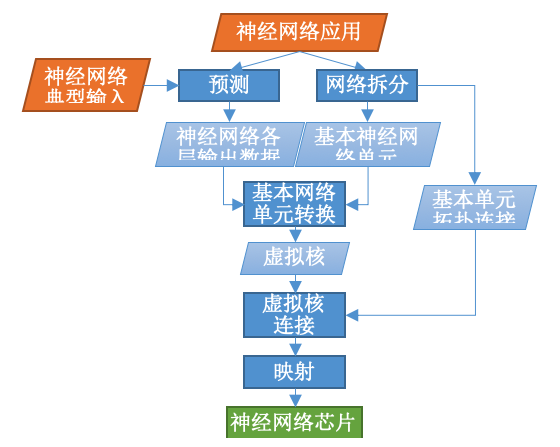
\includegraphics[width=0.60\textwidth]{Img/Chap_Application/Zhang/Systemflow.png}
    \bicaption{系统流程图}{系统流程图}\label{fig:Systemflow}
\end{figure}


\begin{itemize}
    \item 基本神经网络单元\\
    如图\ref{fig:NNUint},基本的神经网络单元为输入为n个神经元,输出为m个神经元,输入神经元与输出神经元之间全相联,若不是全相连,可以以将未相连的边看作连接权重是0的边。通过将复杂神经网络拆成基本神经网络单元,再通过对基本神经网络基本单元的转换,完成对整个神经网络的转换。
    \item 基本神经网络单元的转\\
    神经网络芯片的处理核的功能通常也是处理类似图\ref{fig:NNUint}的结构,但通常输入和输出的数量是固定的,例如IBM的TrueNorth芯片,其神经突触核支持的输入和输出数量均为256。但应用层的基本神经网络单元输入输出节点数量通常远大于硬件所支持的输入输出数量。此外,硬件的权重位宽和输入输出数据通常较低,且常常用整数或定点数来表示。此外,硬件所支持的激活函数或神经元模型通常非常简单,且是固定的。因此基本神经网络单元的转换主要需要解决如下3个硬件带来的约束:连接度约束,即输入输出的数量;精度约束,包括权重以及其他参数的精度和输入输出数据的精度;激活函数或神经元模型的约束。
    
    \begin{figure}[!htbp]
    \centering
    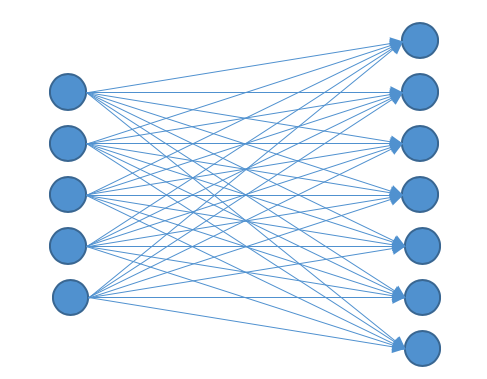
\includegraphics[width=0.60\textwidth]{Img/Chap_Application/Zhang/NNUint.png}
    \bicaption{神经网络基本单元}{神经网络基本单元}\label{fig:NNUint}
    \end{figure}
    
    分别通过权重矩阵稀疏化、低精度训练和插入隐藏层来解决上述三种约束。对基本神经网络单元的训练流程如图\ref{fig:NNUintExchange}所示。

    \begin{figure}[!htbp]
    \centering
    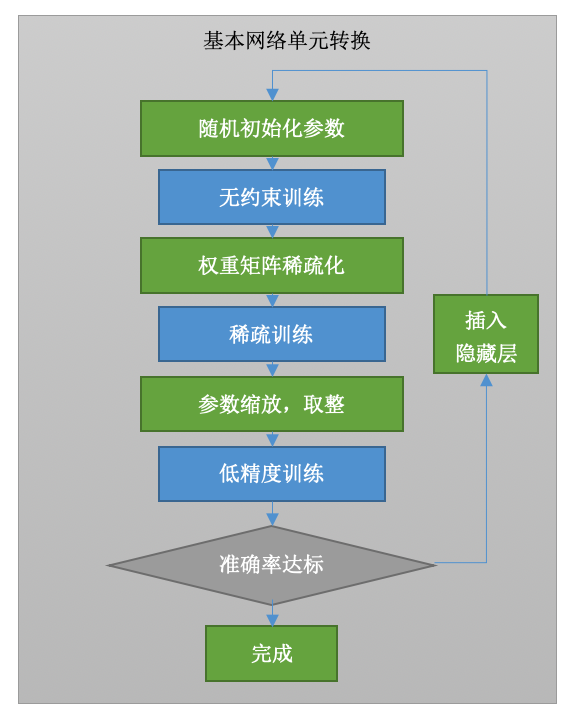
\includegraphics[width=0.60\textwidth]{Img/Chap_Application/Zhang/NNUintExchange.png}
    \bicaption{神经网络基本单元转换流程}{神经网络基本单元转换流程}\label{fig:NNUintExchange}
    \end{figure}

    对于n个输入,m个输出的基本神经网络单元,构建一个输入层为n个,输出层为m个,输入输出之间全相联的神经网络,神经元模型或激活函数使用神经网络硬件所支持的。用基本神经网络单元的典型输入输出数据来训练构建的神经网络。
    
    首先随机初始化参数,不加任何约束地训练这个网络,若硬件所支持的是ANN,则使用经典的随机梯度下降来训练,如果硬件所支持的是SNN,则使用其spike发放频率作为输入输出数据,同样适用随机梯度下降来训练,训练之后使得网络对输入的预测结果与对于的输出尽可能接近。
    
    若n超过了硬件所允许的最大输入k或者m超过了硬件所允许的最大输出l,则进行权重矩阵稀疏化。如图\ref{fig:matrix}所示,在权重矩阵的对焦线上选择一系列子矩阵,使得每个子矩阵的大小均满足硬件的输入输出限制。通过不断交换矩阵的行或列,或者将其中某一行或某一列从一个子矩阵移到另一个子矩阵,使得所有子矩阵中的权重的绝对值总和最大。
    
    \begin{figure}[!htbp]
    \centering
    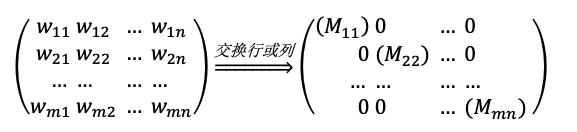
\includegraphics[width=0.65\textwidth]{Img/Chap_Application/Zhang/matrix.png}
    \bicaption{权重矩阵稀疏化}{权重矩阵稀疏化}\label{fig:matrix}
    \end{figure}
    
    经过稀疏化之后,所有子矩阵之外的权重均强制设置为0,并以此为约束重新训练。训练完之后,根据神经元模型,在不影响结果的情况下,将所有的参数线性缩放,使得所有的参数刚好落在神经网络硬件的精度范围内,并四舍五入到硬件的精度。重新训练网络,所有参数在训练时保存为浮点数,在训练前馈过程中,首先将所有参数四舍五入到硬件的精度,在反馈和更新的过程中,使用仍然采用浮点数。
    
    若低精度训练之后,网络的准确率不能达到预期的要求,则在输入层和输出层之间增加隐藏层,重复上述步骤,直到网络的准确率能达到预期的要求为止。
    
    此时得到的网络已经满足硬件的所有约束条件,权重矩阵稀疏化过程中的每个子矩阵看作一个虚拟核,与神经网络芯片中的一个核相对应。
    
    \item 复杂网络拆分和逐层转换
    
    这儿将介绍对于任意的复杂网络,如何拆分成基本神经网络单元。 
    
    \begin{figure}[!htbp]
    \centering
    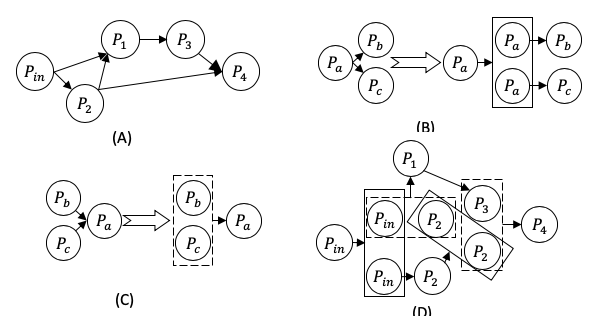
\includegraphics[width=0.60\textwidth]{Img/Chap_Application/Zhang/MNsplit.png}
    \bicaption{复杂网络的拆分}{复杂网络的拆分}\label{fig:MNsplit}
    \end{figure}
    
    复杂神经网络以层为基本单元,每层神经元包含若干神经元,层与层之间相互连接,形成一个有向图,如图\ref{fig:MNsplit}(A)所示。

    对于有向图中任意节点$P_a$,若$P_a$有n个后向节点,则引加入一个多播层$P_na$,该多播层由n个$P_a$拼接而成,如图\ref{fig:MNsplit}(B)所示,$P_a$与$P_na$之间的连接为基本神经网络单元,$P_na$中的每一份$P_a$分别与一个后向节点相连。
    
    对于有向图中任意节点$P_a$,若$P_a$有n个前向节点(已增加完多播层),如图\ref{fig:MNsplit}(C)所示,将Pa的所有前向节点拼接在一起当作一层$P_pre$,此时$P_a$与$P_pre$之间的连接为基本神经网络单元。
    
    经过了上述步骤,可以将复杂神经网络拆分成基本神经网络单元,进而利用前面所述的转换方法拆分成若干虚拟核。例如图\ref{fig:MNsplit}(A)中所示的神经网络被拆分成了图\ref{fig:MNsplit}(D)中所示结构,其中图\ref{fig:MNsplit}(D)种每个箭头表示一个基本神经网络单元。
    
    神经网络的典型输入从输入层输入,在原神经网络的每一层产生相应的输出,为基本神经网络单元的转换提供训练数据。
    
    由于基本神经网络单元的转换会有误差,为了避免误差的逐层积累。对于有向无环图,对图进行拓扑排序,按照拓扑排序的顺序逐层进行转换,每个基本神经网络单元转换完在之后,利用其输入和训练出的权重等参数生成其输出,并以该输出作为后续基本神经网络单元训练时的输入数据。对于有环图,切断其中若干条边使得图中所有的环消失,然后对其进行拓扑排序,并按照该顺序进行基本神经网络单元的转换,若基本神经网络单元的部分输入来自切断的边,则利用原神经网络每一层产生的输出作为这部分输入的数据。
    
    \item 虚拟核的连接和映射
    
    经过上述步骤,复杂神经网络被拆分为基本神经网络单元,并按照拓扑排序的顺序进行逐层转换,最终得到了若干虚拟核,根据拆分和权重矩阵稀疏化步骤的连接信息,将这些虚拟核连接起来,得到虚拟核的连接图,利用经典的片上网络的映射算法(例如KL算法)将虚拟核与芯片上的物理核一一对应,将各个虚拟核的参数配置到对应的物理核上,完成神经网络的转换。
    
    \item 神经网络编译精度\\
    (补充数据)

\end{itemize}

(2)支持基本神经网络单元的可重构神经网络加速器设计

(1)中引入了神经网络和芯片之间的数据流图形式的中间层,中间层的计算单元是基本神经网络单元,该单元的计算主题是向量矩阵乘,因此证明这一软硬件去耦合设计思路优越性的关键是能否设计支持这类基本神经网络单元的高效加速器结构,尤其是考虑到(1)中的神经网络编译会增大神经网络的规模,这就使得支持基本神经网络单元的高效硬件设计尤为重要。

本节基于具有高密度、高能效向量矩阵乘计算能力的ReRAM交叉开关结构,同时针对神经网络内部的数据通信特性提出采用可重构片上互连机制,并引入可重构逻辑实现数据流计算图的片上控制功能,从而提出可重构神经网络加速器设计,称为FPSA(Field Programmable Synapse Array)。

仿真测试表明,该设计的网络推断性能较同样基于ReRAM交叉开关结构的PRIME加速器结构提升1000倍。

\begin{itemize}
    \item ReRAM与基本神经网络单元
    ReRAM(resistive random-access memory,非易失性阻变存储器)是新一代的多级(Multi-level)存储器件,理论上可以将ReRAM的电导值设为其取值范围中的任意值。我们可以将ReRAM在Crossba交叉点的阻值设置为神经网络权重矩阵的对应值,这样就可以用一个ReRAM Crossbar来表示一个神经网络的权重矩阵,并且根据其物理特性就地(in-situ)完成矩阵向量乘操作。对于理想的Crossbar器件,将输入电压$V_i$加到每一行(字线,word-line),电压与每一交叉点的电导值$G_ij$ 相乘,根据基尔霍夫定律$I=GV$,每一列的输出电流$I$ 可累加得到,该计算过程能达到很高的并行度和速度。本设计中就是以高密度、高能效的ReRAM交叉开关结构作为基本神经网络单元的基础实现。(附图)
    
    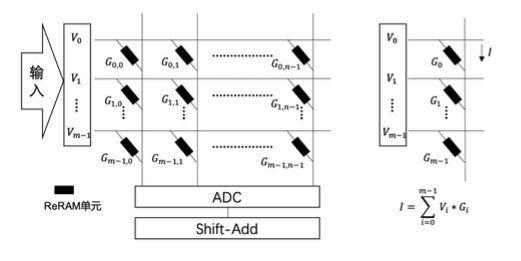
\includegraphics[scale=0.6]{Img/Chap_Application/Zhang/ReRAM.png}
    
    \item 可重构神经网络加速器结构设计\\
    
    With the hierarchical software system, we propose the compact and efficient FPSA architecture. FPSA is a reconfigurable architecture composed of three kinds of functional blocks: ReRAM-based PE, Spiking Memory Block (SMB), and Configurable Logic Block (CLB). ReRAM-based Processing Element (PE). Due to the transformation of neural synthesizer, the PE only needs to support the HEM IR with ReRAM-crossbar. To further reduce the overhead of ADC/DAC, we employ spiking schema, which uses the spike count of 1-bit spikes to represent input/output data. And the corresponding ReLU function can be implemented with a simplified Integrate-and-Fire (IF) neuron model. We propose a compact circuit design to enable core-op computation with the spiking schema.
    
    Spiking Memory Block (SMB). Since PEs communicate with 1-bit spikes, we propose SMB to buffer the information. It integrates the spike counter and generator together with the memory array to enable efficient load and store of spike counts. Configurable Logic Block (CLB). As mentioned above, to enable flexible and temporal scheduling of the spatial-to-temporal mapper, we introduce CLB widely used in FPGA to implement control logic. Till now, FPSA provides massive functional blocks for the software system. Further, to match the high throughput of PE, we use a reconfigurable routing architecture composed of plenty of wiring resources and configurable switches to connect these functional blocks together.

    Accordingly, neural synthesizer, one tool of the proposed software system, can convert an NN in the SPM form into an equivalent CG of core-ops. Thus, we can support NN frameworks flexibly and the hardware only needs to support core-op, which greatly simplifies the circuit design of FPSA. Further, we integrate reconfigurable buffer resources and control logic in hardware and introduce a spatial-to-temporal mapper in software. The latter schedules the execution of HEM and turns it into a netlist composed of the PEs, the buffers and control logic. Finally, to match the high throughput of the ReRAM-based PEs, we propose a reconfigurable routing architecture as the interconnection subsystem to supply extremely high bandwidth and low latency. At the same time, a placement \& routing tool is leveraged to place the netlist onto hardware and generate the routing configuration.

    Compared to one state-of-the-art ReRAM-based NN accelerator, PRIME [9], our approach improves the performance by up to 1000× for representative NN models and the accuracy loss is negligible. 
\end{itemize}

(参考文献:Bridging the Gap Between Neural Networks and Neuromorphic Hardware with A Neural Network Compiler,ASPLOS 2018论文;

FPSA: A Full System Stack Solution for Reconfigurable ReRAM-based NN Accelerator Architecture,ASPLOS 2019论文)

\subsection{相关工作}
(根据上述具体工作再做相关展开)
